\documentclass[whitecover]{MO_report}
\usepackage{graphicx}
\begin{document}

\title{Thea Design Document}
\author{Michael Walker}
\maketitle

\tableofcontents

\pagebreak

\chapter{Introduction}

Cubeviz is a lightweight visulisation GUI for use with Iris and Cartopy.

Cubeviz enables the user to load cube lists from file, using the load method
from iris, and select an individual cube from the list. It will then
extract and plot 2-dimensional slices of this cube according to the user's
choice of dimensions to collapse and the points to collapse the dimensions
onto.

The program gives a range of options for how the slice should be plotted,
including the option either to rapidly plot straight from the data or to use
the slower but more powerful iris tools, and is
able to provide feedback on the plotted cube by showing the summary of both the
full cube and the current slice, as well as a table of the data contained
within the slice.

Finally, an image of the plot can be saved in numerous formats and if you would
like to adapt the image or show how the image is created, you can view
source code for the plot, which you are also able to save in numerous formats.

\vspace{4mm}

The GUI has been written in Python, the interface was designed in Qt
Designer, and built using Qt4 with the PySide binding. (see chapter 8 for more
details)

\pagebreak

\chapter{Brief}

\section{Goal}

The goal of the project is to allow a user to visualise an Iris cube, 2D slice
by slice, by using a python GUI application.

\section{Scope}

This project is to create a lightweight python application that permits a user
to visualise data using Iris (and Cartopy). The project code name is 'thea'.

\vspace{4mm}

The scope of the project includes:

\begin{itemize}

\item
Gather user requirements and break them down into 'must have', 'should have'
and 'could have' priorities.

\item
Analyse the requirements (functional and non-functional) into a set of
development tasks. Analysis will also include some prototype storyboards of
the GUI layout;

\item
Justification of the GUI design pattern used.

\item
Development of the GUI using an open sourse repository (GitHub). Source code to
be written in Python using PySide.

\item
A set of tests to excercise the model and controller component of the selected
design pattern

\item
Iteratively work with the identified end-user;

\item
Documentation on design and use of the GUI.

\item
A presentation of the project outcomes

\end{itemize}

\section{TimeScale}

This project may last for up to three months, including early investigations
and final write up.

\section{Underpinning Technology}

The project should make use of Python tools provided for Met Office Science.

\section{Deliverable}

\begin{itemize}

\item
A working GUI that visualises data using Iris and Cartopy.

\item
Documentation on the design

\item
User Documentation on how to use the GUI.

\end{itemize}

\section{Sample Data}

Sample data can be found in the Iris test repository
(https://github,SciTools/iris-test-data).

\section{Project Extensions}

If time permits then additional features can be added as prioritied by the user
and if the capability is availiable in the underlying libraries. Such features
could be:

\begin{itemize}

\item
User choice of color palette

\item
User choice of projection

\item
Gridlines on or off

\item
Export of the rendered image to an image file.

\item
User choice of phenomena to slice over.

\item
Export sourcecode to generate image.

\end{itemize}

\section{Reference List}

\begin{itemize}

\item
http://zetcode.com/gui/pysidetutorial/

\item
http://en.wikipedia.org/wiki/PySide

\item
http://www.codeproject.com/Articles/228214/Understanding-Basics-of-UI-Design-Pattern-MVC-MVP

\item
http://www.codinghorror.com/blog/2006/01/visual-design-patterns.html

\end{itemize}

\pagebreak

\chapter{User Requirements}

Although I worked with and recieved feedback from several people during this
project, the indentified end user was Dr Kerry Day.

In the first meeting with Kerry, which occured on 09/07/2013, I presented her
with a very early draft of the GUI, which was able to load a cube list, allow
you to select a cube from the list and then plot simple 2D cubes. It displayed
the plot by first saving the plot to file and then printing the image to the
screen (as a method for embedding matplotlib had not yet been found)

As a result of this meeting, and the further meetings that followed as the
project progressed, the goals for this project became defined:

\vspace{4mm}

\section{Must Haves}

\begin{itemize}

\item
Ability to load cubes from file.

\item
Ability to extract a 2D cube to plot from a larger cube.

\item
Be able to plot the 2D cube.

\item
To be able to step through slices in the cube.

\item
Option to save the generated plot.

\item
Option to display the data in the cube.

\end{itemize}

\section{Should Haves}

\begin{itemize}

\item
To be able zoom in on areas of the graph

\item
Ability to mark on political boundaries

\item
Range of different plot types

\item
Range of different color schemes

\item
Option to add grid lines

\item
Label all axes.

\item
Option to set a colorbar over the entire set of slices and not just the current
image.


\end{itemize}

\section{Could Haves}

\begin{itemize}

\item
Code Generation

\item
Option to add met office logo

\item
Colorbar resizes to same length as image.

\item
Choice of projection

\item
Ability to specify the range over which the colorbar was set.

\item
Options for plotting in 3D

\end{itemize}


\pagebreak


\chapter{Design}

From the start of the project, it was clear there were three main roles that
the interface needed to fulfill. The first, was some way to show the plot from
the cube, secondly, there would need to be a section which displayed information
about the cube, and thirdly, there must be some way for the user to make
decisions about what to plot.

Initialy, while the focus was on functionality, a simple setup was used with
the left of the screen divided vertically between the image and the summary of
the cube, and the right of the screen being devoted to the options.
A menu system was also put in place, providing the save and load options, as
well as an alternate method of making choices.

\begin{figure}[ht!]
\centering
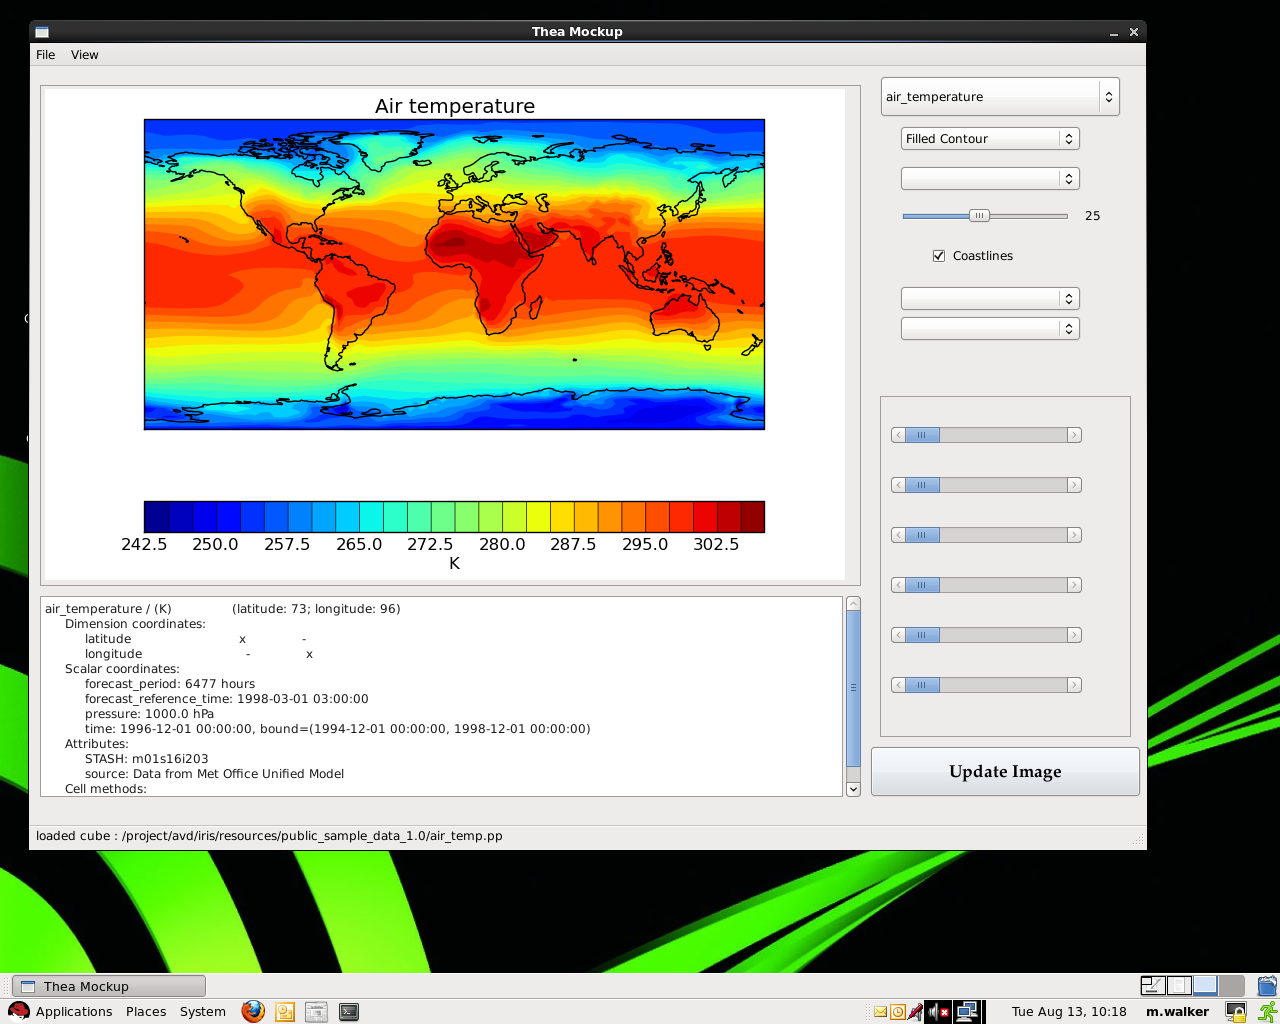
\includegraphics[width=100mm]{version1.png}
\caption{This early draft had a similar overall layout to the current design,
but had limited functionality, and could not be resized.}
\label{overflow}
\end{figure}

Even with this early draft, it became apparent that due to the time taken to
redraw the plot as each change was made, it was taking too long to make
multilple changes to the plot. Furthermore, because Qt locks the interface
while the calculations are being done, this was introducing a large amount of
lag into the interface. (See section 8.4 for details) Ideally, it would be
possible for the program to run the caluculations in background, thus leaving
the interface free from lag, while still updating the plot. However, due to the
way that Qt handles events, this is diffucult to achieve. As a result of this,
the graph is now only redrawn when the update button is pressed (or next and
previous slice buttons), or when a new file is loaded. This allows the user to
change as many of the options as desired without any lag, before replotting the
image.

While I felt that elements of this setup worked very well, (the left of the
screen for example is still divided between plot and information with options
to the right), as more options were added this became increasingly messy, and
the menu layout began to feel slow and clunky.

At this stage, with the many of the technical challenges overcome, a
reworked design was required.

\begin{figure}[ht!]
\centering
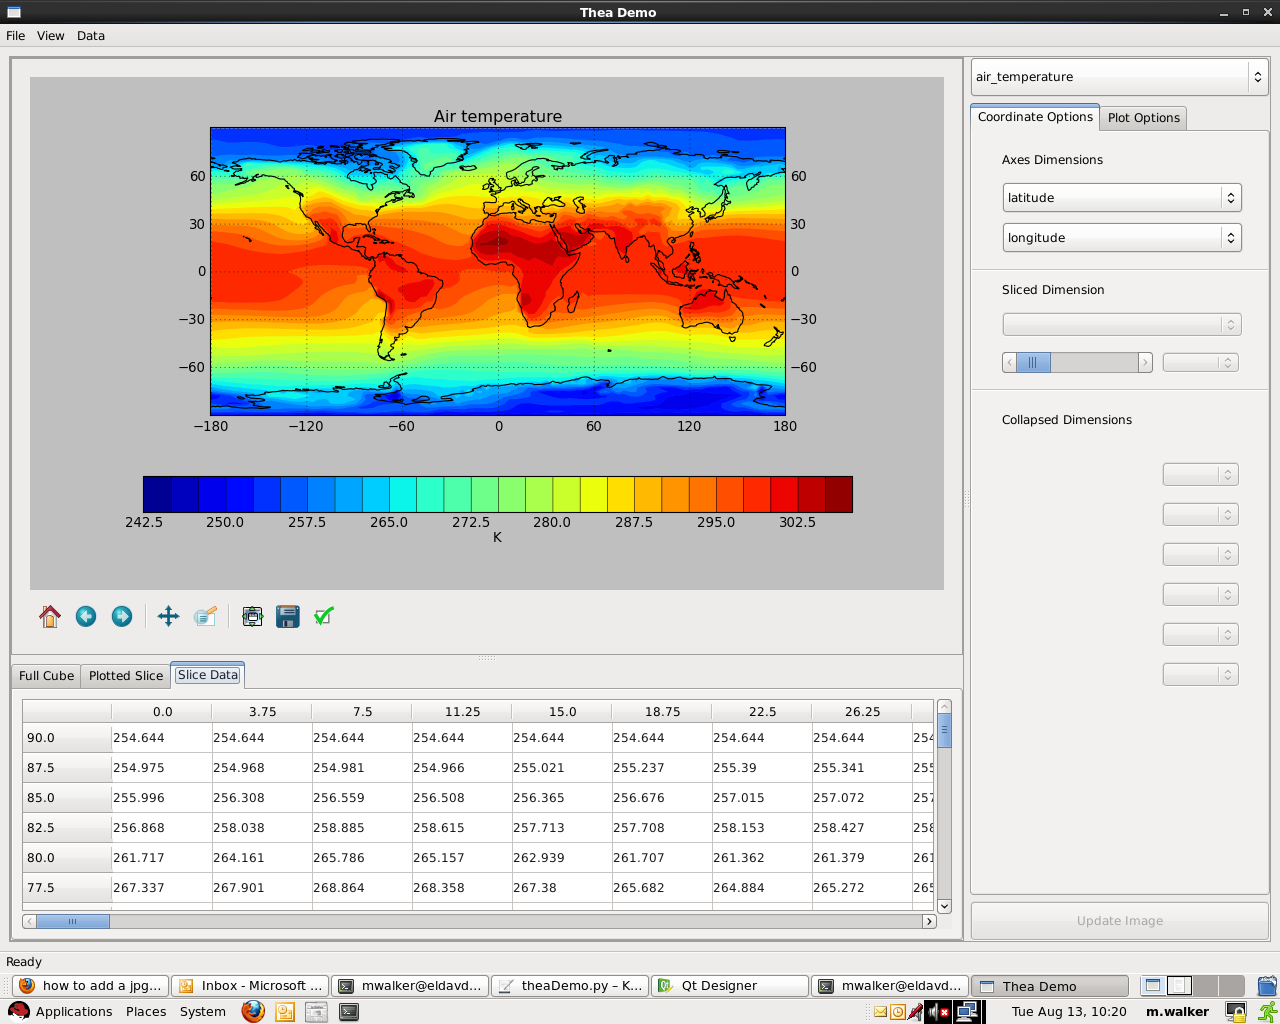
\includegraphics[width=100mm]{version2.png}
\caption{As more buttons were added, a tabbed browser was used to sort the
options.}
\label{overflow}
\end{figure}

\vspace{4mm}

My first thought was to divide up the sections. The cube information section
was split into two tabs, one containing the summary of the original cube,
and the other containing the summary of the plotted slice. This worked nicely
and is still used. The options were then split into those concerning the
dimensions, and those concerning the plot options and again placed into
separate tabs. The menu bar remained unchanged.

A major breakthrough was to use the vertical and horizontal splitters in
combination with layouts to make the interface resizable. The splitters
had the added advantage that sections of the screen could be dragged out of
the way, giving more room to the other elements

While this made for a much tidier interface, when using it I felt that I was
having to switch tabs too often and it was too slow to reach the options that
I wanted.

\vspace{4mm}

\begin{figure}[ht!]
\centering
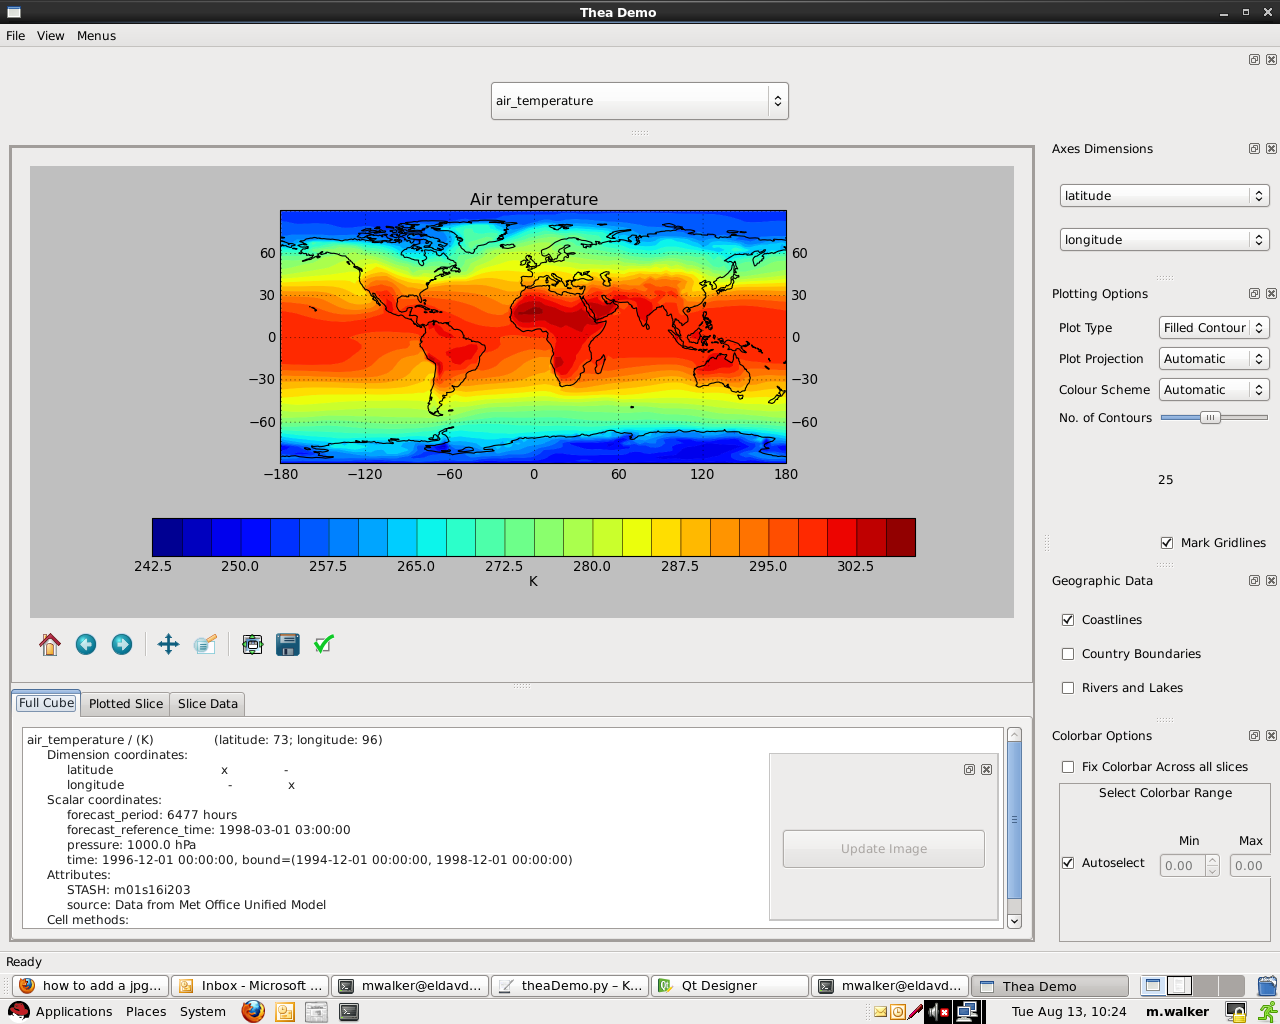
\includegraphics[width=100mm]{version3.png}
\caption{The use of docked widgets gave a lot of freedom, but added too much
complexity.}
\label{overflow}
\end{figure}

My next step was a play with the dock widgets availiable in Qt Designer.
These widgets can be attacted to window, moved around, dragged ontop of one an
other to form tabs between the two widgets and could be opened and closed
individually.

The hope was that I would be able to brake the interface down into
small groups of a few related options, and then be able to choose which options
you wanted on screen and where and how you wanted them to be displayed.

I made a quick demo of this as shown, and while it had some nice properties
(the right hand side of the interface in Qt Designer itself uses these to good
effect), it ended up feeling much too involved and complicated for a lightweight
application such as this.

\vspace{4mm}

As I began to like the menubar less and less for this project, due to the need
to press a minimum of 2 buttons to do anything, and the fact that I was unable to
control the size of the buttons, forcing them to be small and so slow to use, I
began to look for other alternatives.

In the end, I settled on the toolbar. This can be resized, and icons can be
used to reduce the amount of text onscreen. Initialy, I was intending to
make the buttons on the toolbar each open a dialog box, but I soon realised
that while this was great for the load and save buttons, for much of the rest
of the options, I could pin the options themselves to the toolbar.

\begin{figure}[ht!]
\centering
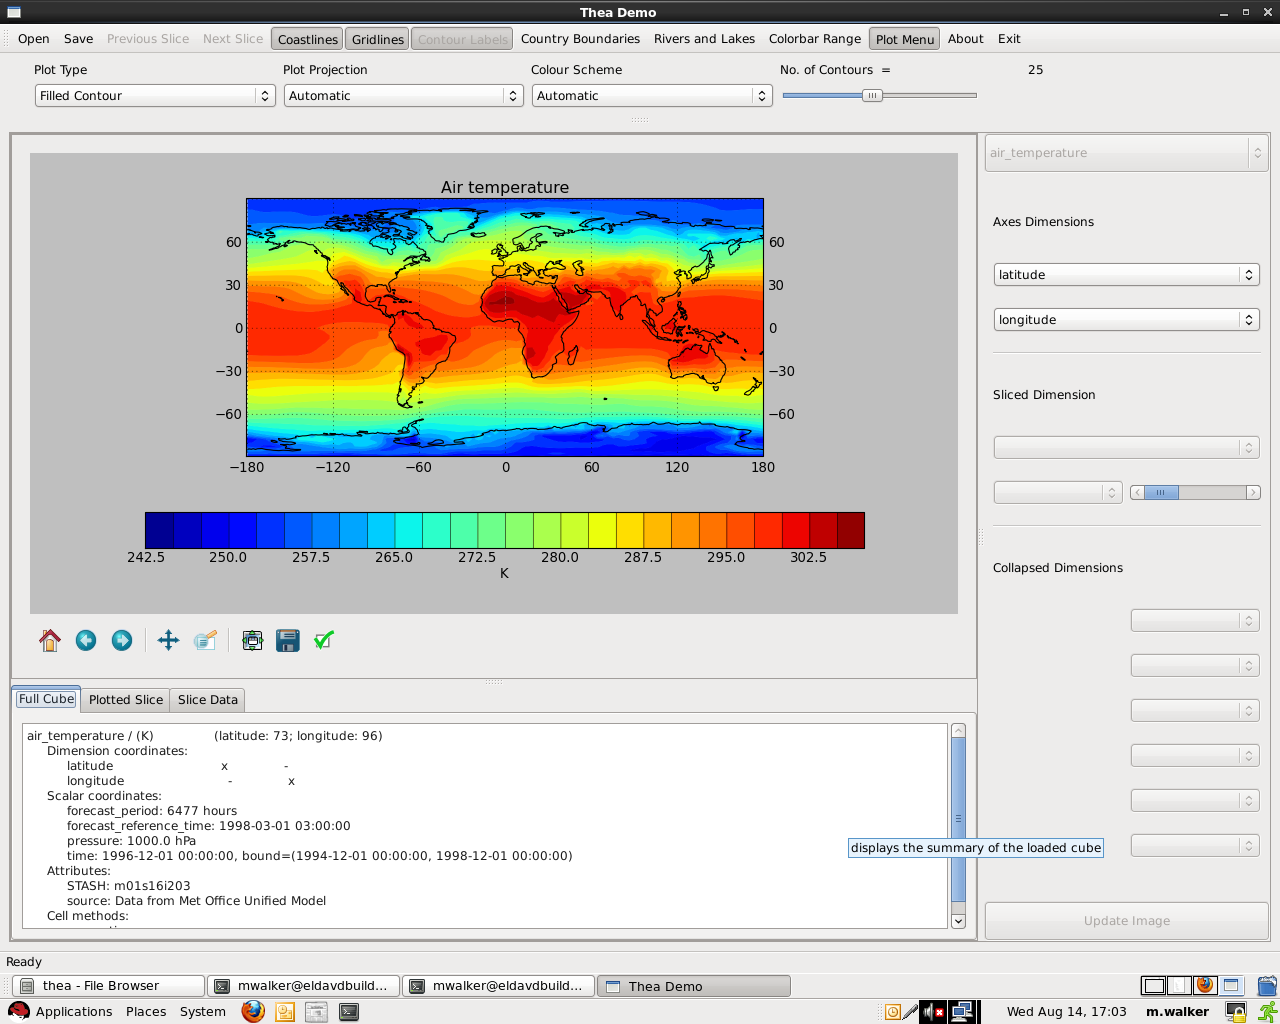
\includegraphics[width=100mm]{basic.png}
\caption{The use of the toolbar allows for all of the options to be on screen
at once, and the abilty to drag components in and out of the screen maintains
flexibility.}
\label{overflow}
\end{figure}

When this was combined with a fixed dock widget bellow it, I had an interface
in which almost all of the options were accessable with a single click, and
via a shortcut, and each section could be dragged on and off of the screen as
required.

The final major improvement to the interface was the ability to dynamocally
generate buttons. This allowed me both to reduce the clutter due to unused
buttons in the collapsed Dimensions section, and to allow in theory for an
unlimitted number of dimensions to be handled. (In practice I have been unable
to make the collapsed dimensions produce a scroll bar when there are too many
to fit on the screen and so instead the window expeands, even beyond the size
of the screen with enough dimensions, making the size of the monitor the
limmiting factor)

With the final development, we arrive at the current design for the interface,
seen below.

\begin{figure}[ht!]
\centering
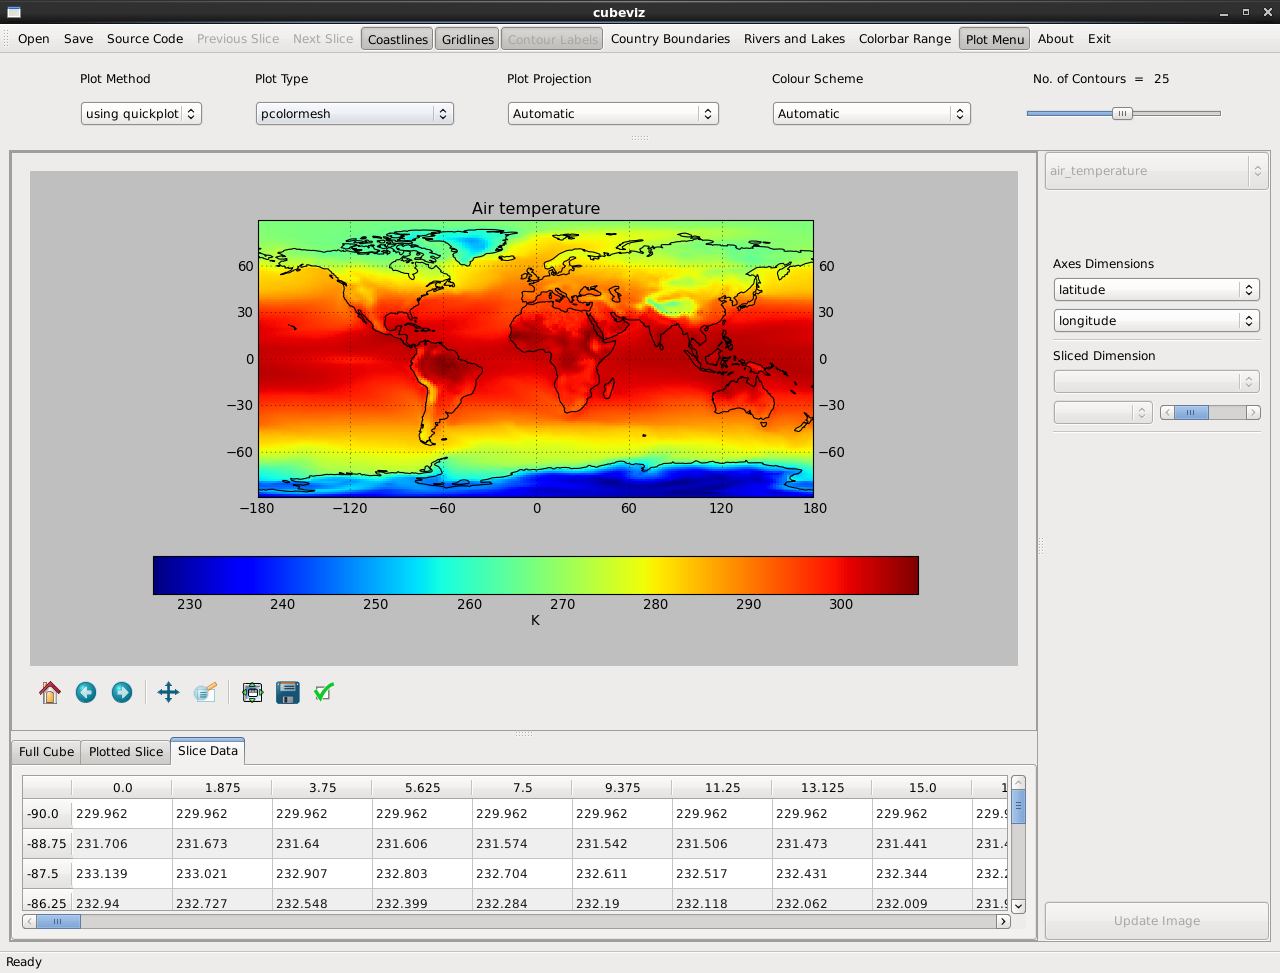
\includegraphics[width=100mm]{tutorial8.png}
\caption{The current main window.}
\label{overflow}
\end{figure}

\pagebreak

\chapter{Technical Challenges}

In this section, I outline the main technical challenges that were faced in the
making of the application, and the methods currently used to solve them.

\section{Embedding Matplotlib}

By far the largest challenge faced, was how to get matplotlib working inside my
mainWindow. This was a highly desirable goal, as many of the requirements of
the project would be solved imediately by use of the interaction with the plot
that matplotlib provides. For example, it would allow for zooming to a specified
region of the plot. The second advantage,
was that it got rid of the process of saving an image to file and then fetching
it back, which seemed iniefficient. Finally, it gave users a familiar look
and control interface to work with.

In order to embed matplotlib in PySide, we must first change the backend of
matplotlib to be Qt4Agg. This can be done as follows

\begin{verbatim}
>>> matplotlib.use('Qt4Agg')
\end{verbatim}

By default however, this backend will use the Qt4 binding and not the PySide
binding that we are using. To change this, we must change the settings in
matplotlib. This can be done programatically using the command

\begin{verbatim}
>>> matplotlib.rcParams['backend.qt4'] = 'PySide'
\end{verbatim}

Having switched the backends, we can then create a canvas for the plot to be
drawn to and embed that into our application as described in section $7.4$.

\section{Extracting an Arbitary Cube}

Iris provides several methods for extracting cubes. The methods that I
considered using for this application were slices, constraints, and indices.

The inputs that would be most easily given to the function would be the name
of the dimensions to work with (fetched from the select dimension boxes) and
the index of the point in each coordinate to collapse onto (taken from the
index of the corresponding combo box)

I began by using slices, as it provided a very simple method for returning a
2D cube. However, it quickly became apparent that this method would not scale
easily to obtaining a specified slice from a large cube as, due to its nature as
an iterator, it would have to cycle through a large number of slices until it
found the correct slice.

The next attempt was to try to use constraints. This had the advantage that it
would return a specific cube, but was made very tricky by the fact that this
method takes in the values within a coordinate to collapse around instead of
the index of a coordinate. The value of the coordinate at any given index point
can be easily found using coord(coordName).points[index], but then, due to
the value being a floating point value, some simple bounds had to be created
around this value to avoid the constraint excluding the desired value. Even
after this, this method was very unreliable for data which contains bounds.

It was now apparent that the index of the coordinate was going to be the only
reliable mathod for this purpose, and at this point, it was suggested to me
that I would be able to use the index notation method to do this. The
implimentation of this method is best seen through an example.

Imagine a 4D cube, with dimension coordinates [time, height, lat, lon], and
lets imagine that time coordinate has points [6,7,8,9,10,11] and that the
lon coordinate has points [150, 155, 160, 165].

If then, we wanted to extract the 2D cube, which has time 7 and lon 160, then
we would normally be able to do this with the following code.

\begin{verbatim}
>>> sub_cube = cube[1,:,:,2]
\end{verbatim}

This is exactly what we would like to recreate, and can be done by creating as
many slice objects as we have dimensions. This is done with:

\begin{verbatim}
>>> slices = [slice(None)] * cube.ndim
\end{verbatim}

Applying this would be equilalent to

\begin{verbatim}
>>> sub_cube = cube[:,:,:,:]
\end{verbatim}

From here, we can simply loop over the coordinates, changing the slice(None)
object to an index where required, and then extract the sub-cube using:

\begin{verbatim}
>>> sub_cube = cube[tuple(slices)]
\end{verbatim}

This method has worked well consistently, and even works for collapsing
anonymous dimensions.

\section{Producing the Data Table}

The data table was requested so that when points in the graph looked suspicious,
users would be able to quickly refer back to the raw data in order to get a
better idea what has happening.

The data table went through numerous iterations. Initially, the thought was
simply to print out the data of the cube, and then to think about some way
of formatting the data into a more presentable table. However, the formatting
would have been quite complex to get right for a general data shape, and the
results were not especially fast or attractive.

The next step was to try to use the inbuilt QTableWidget from Qt. This worked
very nicely for slices with a small amount of data, producing a smartly
presented table. However, for the larger data sets, the table very quickly
became prohibitively slow. For this reason, I decided to switch to using a
QTableView object instead. This differs from the QTableWidget because it does
not deal with the data itself. Instead, a custom model must be created which
has access to the data and will pass the correct data to the QTableView as it
is requested. This method proved far faster than the QTableWidget, while still
retaining the presentation. For more information about the QTableView object
and the tableModel class, see section 7.4.

\section{Working with cubes containing anonymous dimensions}

As I began to test the application on a wider range of cubes, I came across a
couple which I was not able to display. On closer inspection of these cubes,
it turned out that the reason for the failure was that they possessed anonymous
dimensions. (Examples of such cubes are NAME\_output.txt in Iris Sample Data
and the ORCA2 data.) This caused problems as many of the methods in the application
made use of the names of the dimensions to identify them. Almost all of the
methods have now been changed so that they now idetitfy dimensions by other
means, and the program now includes the anonymous dimensions when it fetches
the list of names. One method remains however which still requires the
coordinate itself is the coord(coordName).points method. This is used both to
get the list to populate several of the combo boxes, and to populate the
headers in the table. Anonymous Dimensions do not contain this information
however, and so instead I have chosen to catch the coordinateNotFoundError
that is produced in this case and to simply use the index of the points instead.


\pagebreak


\chapter{Class Hierarchy}

\section{Directory Structure}

For reference, I include a list of the directory structure used.

\begin{verbatim}

<basedir>
    |
    + <docs>
    |   |
    |   + design_doc.tex
    |   + design_doc.pdf
    |   + user_manual.tex
    |   + user_manual.pdf
    + <lib>
        |
        + <thea>
            |
            + <generated_code>
            |   |
            |   + __init__.py
            |   + about_dialog_layout.py
            |   + about_dialog_layout.ui
            |   + colorbar_dialog_layout.py
            |   + colorbar_dialog_layout.ui
            |   + main_window_layout.py
            |   + main_window_layout.ui
            |   + source_code_dialog_layout.py
            |   + source_code_dialog_layout.ui
            |
            + <tests>
            |   |
            |   + __init__.py
            |   + test_cube_logic.py
            |   + test_gui_logic.py
            |   + test_main_window.py
            |
            + __init__.py
            + about_dialog.py
            + colorbar_dialog.py
            + cube_logic.py
            + gui_logic.py
            + main.py
            + main_window.py
            + matplotlib_widget.py
            + source_code_dialog.py
            + source_code_generator.py
            + table_model.py

\end{verbatim}

\section{The Big Picture}

When the main method is run, it first creates a QApplication instance. This is
required for any program using Qt as it contains the main event loop for the
program. More information can be found here:

\begin{verbatim}
http://harmattan-dev.nokia.com/docs/library/html/qt4/qapplication.html
\end{verbatim}

It then creates an instance of the MainWindow class. This is the top level
class in the program. (More information in section 7.1). The MainWindow
class is responsible for displaying the information and plots of the cube,
controling the objects contained within the main window and for collecting
information about choices made by the user. 

From this class, further dialogs are called as required, and the libraries that
have been created can be called apon to carry out calculations that are needed.

The files found in the $generated\_code$ directory are files that have been
created using Qt Designer. The .py files here are used to set up the inital
layout of each of the respective windows and dialogs, placing objects onto them,
and defining their initial properties. For more about the generated files, see
section 7.6.

Tests for the program can be found in tests directory.


\pagebreak


\chapter{Breakdown of Files}

\section{main\_window}

This file contains the MainWindow Class.

This class has 3 main roles:

1) Defines the reasponse to events in the MainWindow.

2) Reads data from and writes data to objects contained within MainWindow.

3) Controls which of the options are enabled at any stage.

\vspace{4mm}

1) PySide has a signal and Slot model for events (see section on PySide for
more details). The Main window class sets up what the slots are, and which
signals are connected to them. Using this method, we define how the MainWindow
interacts with the user. 

2) The MainWindow class is the only class which has access to the objects
within the MainWindow. As such, much of the code in this class is
involved with either fetching information from the objects (such as whether or
not the user wants coastlines to be plotted or which dimensions are being
plotted) and passing it to the relevant methods, or getting information from
the functions and writing that into the objects to be displayed.

3) Not all options are availiable all of the time. For example, trying to plot
coastlines on a plot of height against time, will result in an error. Therefore,
to prevent this possiblility, the coastlines option will be disabled in this
case. As the MainWindow class is the only class that can access the objects,
they are enabled and disabled from within this class.

\section{Libraries}

\subsection{cube\_logic}

This file contains a library of functions for performing calculations on the
cube. The largest section of code here is the update method, which allows for
the reduction of a cube from N dimensions down to 2, and the creation of a plot
object for a cube. (This method is not involved with actually rendering the
cube)

These functions were separated from the mainWindow code to make the code more
modular, and easier to test. Before this, these functions collected information
directly from the interface from within the function. This meant that it was
almost impossible test them, as very few of the variables they required were
entered as arguments.

\subsection{gui\_logic}

This library contains the functions used to decide was information should be
displayed by the interface. The main roles are to obtain data from the cube,
that is require to populate the comboBoxes, and to make descions about which
elements in the interface should be enabled at any time.

\subsection{source\_code\_generator}

This file contains a function which is able to create source code that would
reproduce the current plot. It takes a dictionary containing the state of the
main\_window as an argument, and then returns a formatted string representing
the source code.

\section{matplotlib\_widget}

This file contains the MatplotlibWidget class, and is how we are able to
embed matplotlib into a Qt window. 

When we created the main\_window in Qt, we included in it a custom widget
which we named matplotlib\_display. We were then able to manipulate this
widget as any other object during the design.

We now needed to define how this widget would function, and this is where the
MatplotlibWidget class comes in. We define the matplotlib\_display to take its
instructions from this file, and then define this to functoin as follows.

We first create a figure object using the get current figure command, gcf().
If there is a figure being used at the time, then it will use this, if not,
it will create its own, blank, figure.

We now create a matplotlib FigureCanvas object. This is a class within
matplotlib, and is effectively a canvas onto which we are able to draw our
plot. When we call this, we set it to display our figure.

Finally, we can create a layout, add the canvas to the layout and apply the
layout to the widget.

To update the plot, we simply set the figure to be the new plot.

\section{table\_model}

This module contains the TableModel class.

The TableModel class is my custom model used by the QTabelView object in Qt.

The aim is to be able to provide a table within the main window that displays
the data contained within the current slice.

For more information on the model-view approach, see
\begin{verbatim}
http://qt-project.org/doc/qt-4.8/modelview.html
\end{verbatim}

For more information on the QTableView object, see
\begin{verbatim}
http://harmattan-dev.nokia.com/docs/library/html/qt4/qtableview.html
\end{verbatim}

This model is designed to work with the data of the cube, such that it is able
to pass to the QTableView object all of the data that it asks for.

To do this, it has to be able to supply the number of rows and columns that
will be needed for the table, the data to fill the row and column tables, and
the data required to fill the cells in the table.

\section{Dialogs}

The following modules all provide a setup for their respective dialogs. They
all make use of generated code to provide a layout for the dialog box and set
some of the initial properties. For more information on the generated files,
see section 7.6.

Some of the dialogs used in the program will not be found here. This is because
there are some inbuilt dialogs, such as the save and load dialogs, which are
provided with Qt. In these cases, I have used the inbuilt classes.

\subsection{about\_dialog}

This file describes a dialog box which displays text information about the
program. This information includes the lisence and where to find help.

\subsection{colorbar\_dialog}

This module contains the ColorbarOptions class. This class describes a dialog
box which provides options about how the range of the colorbar should be
decided. By the range of the colorbar, I mean the values between which the
colors should be spread. For example, using the default colors, we might have
a colorbar defined with blue at 250, and red at 320. There are three options
given in this dialog.
\begin{itemize}

\item
\emph{Automatic:} The Colorbar is defined between the minimum and the maximum
values of the data in the current slice.

\item
\emph{Fixed Colorbar:} The Colorbar is defined between the minimum and the
maximum values of the data across all slices along the sliced dimension.

\item
\emph{Manual:} The Colorbar is defined between two points specified by the
user. 

\end{itemize}

For more detailed information about how the Fixed Colorbar works, see section
$===$

\subsection{source\_code\_dialog}

This file contains the Viewer class, which provides an interface in which the
user can view the genrated code. You are able to copy code from this window
to paste into and other program, or you can save the code as a file.

\section{generated\_code}

In this directory, you will find all of the code required to define the layout
and properties of the windows and dialogs. You will also notice that each file
is saved both in .py format and in .ui format.

The reason for this is that this code originates from Qt Designer. Here, you
can build a window by dragging and dropping components into place. Saving the
resulting design results in a .ui file, and these files can be opened within
Qt Designer in order to edit the design. To use these designs in our program
however, we must convert them into python code. This process is described in
section $===$. The resulting python code is what you see here. 

\pagebreak


\chapter{Qt and PySide}

Qt is an open source, cross platform GUI toolkit, which can be downloaded from

\begin{verbatim}
http://qt-project.org/
\end{verbatim}

PySide is a free software, python binding of Qt. Other alternatives to this
include PyQt, PyGTK, wxPython and Tkinter.

\section{General Impressions}

In general, I have found these tools to be simple to use, well documented, and
powerful enough for the design of this appliaction.

The list of prebuilt components in Qt has been sufficient for everything except
for the embedding of matplotlib and the data table, with numerous buttons,
input methods and methods to display information provided. In particular, more
complex structures like toolbars, menubars and statusbars help to give a more
professional feel with little effort. Documentation on all of the components
can be easily found online, and has always provided me with plenty of
information.

Combined with the drag and drop interface of Qt Designer, I found that I was very
quickly able to create a rough mockup of the application with a good portion
of the functionality.

Another feature that added greatly to the speed with which I was able to
construct the application was the stock dialogs in Qt. Being able to just use
the load and save dialogs saved a great deal of time and effort. 

Getting the components to rescale and reposition with the size of the window
can be done by using layouts. I found that these were time consuming to get
right, especially if you wanted something more complex than the simple grids
provided. Eventually though, by using a combination of splitters and layouts,
I was able to obtain more or less what I was aiming for.

Other slight frustrations were that I would have liked to place buttons right
along the edge of the screen without any pixels inbetween, as this makes it far
faster for the user to be able to move the mouse to the button. However, this
does not seem to be possible in Qt. 

I found the following tutorial for learning the basics of Qt and PySide
(without Qt Designer) can be found here:

\begin{verbatim}
http://zetcode.com/gui/pysidetutorial/firstprograms/
\end{verbatim}

\section{Converting .ui files to .py files}

One complication to using Qt Designer with python is that the created code is
not written in python. You must therefore convert the code into python using
a scrpit called pyside-uic. This is included in the PySide build. To use it,
navigate to the location where pyside-uic is kept, and type the following into
the terminal:

\begin{verbatim}
>>> pyside-uic source.ui > target.py
\end{verbatim}

\section{Signals and Slots}

Signals and slots are the method of dealing with events within Qt.

Signals are emitted whenever something interacts with an object within the
application. For example, when a button is pressed, it would emmit the signal
clicked(). Objects like combo boxes have some more complex and some more subtle
signals. For example, they have signals such as currentIndexChanged(int),
which encode data with the signal. There are also signals which make the
distinction between a programmatic change to the object and a change made by
the user. For example, currentIndexChanged() will be emmitted for programmatic
changes or for ones caused by the user, but triggered(), will only be emmitted
due to interactions with the user.

\vspace{4mm}

All signals can be connected to slots. Slots are the response to the signal,
and can be stock functions built into the object (can be found in the
documentation for the object) or they can be your own functions.
Slots can take arguments, however in this case they must be connected to a
signal which emits the same argument.

If you are using stock signals and slots, then it is often possible (and fast)
to obtain this functionality via Qt Designer's signal and Slot editor.
This allows you to select the sending object, signal, recieving object and slot
from drop down lists.

More information can be found here;

\begin{verbatim}
http://qt-project.org/doc/qt-5.0/qtcore/signalsandslots.html
\end{verbatim}

\section{Qt Event Loop}

The biggest issue that I ran into whilst making Thea, was that Event Loop in
Qt blocked some of the functionality that I would have liked to add.
The issue is as follows:

When a button is clicked, an signal is sent. However, the window is then frozen
until all of the actions triggered by the signal (slots) have been completed,
meaning that the user will not be able to issue any further commands, and that
the window will not update itself again until everything is finished. (The
one exception to this is that some internal features may continue to run, for
example the status bar updates most of the time and the parent window will
continue to be responsive if a child dialog is called from within it.)
While this causes no problem at all for fast tasks such as changing text in a
box etc, when the event that is triggered is large, such as producing a plot,
this can be a pain. It would have been nice, for example, to be able to remove
the update button, by allowing the calculations to be done in background, while
the user continued to use the program. It would also have been nice to concider
the possiblility of animation effects, however as the window does not update
whilst running the animation, this is difficult.

This issue could be sloved by dealing with threads myself, however I have not
touched on this as yet.


\pagebreak


\chapter{Still Wanted}

This section contains things that have either been suggested to me as
functionality that could be included, or elements that I would like to see in
the program. While many of these are options that could be implimented
without too much difficulty, the scope of this project was for a lightweigh
quick viz tool, rather than for a full Iris GUI. As such, adding too many of
these features would quickly make the code far less easy to maintain, and
would ultimately be counter productive. They are inculded here incase anybody
is interested in building on the current state of the project, with a brief
explaination of why they might be desirable, a brief evaluation of how easy
they might be to include, and any reasons why they are not currently in place.

\begin{itemize}

\item
\emph{Aggregation:} I would like to be able to add other options for how the
cube was collapsed. For example, the option to take the mean of the dimension
instead of a specified value could be very useful. While for most cube this
would be an easy feature to add, it would be very difficult to make this
completly general, as methods of aggregation require the coordinates name as
inputs and so this would not work for anonymous cubes. As such, We would either
have to writer new aggregate functions, or detect the anonymous cube and
disable this option.

\item
\emph{Interaction Between graph and Table:} It was also be a very nice feature
for clicking on a cell in the table to highlight the corresponding region
in the plot. Perhaps more challenging, it would also be nice for clicking of the
plot to highlight the corresponding cell in the table. The signal and slot
concept from Qt would be very well suited to this, and it is not too hard to
mark points on the plot. This is a feature that I would have liked to have
added had I had more time.

\item
\emph{Fix cut-off lat-lon} Currently if the plot is a lat lon plot, the section
of the matplotlib display which prints the cursor position cuts off the
coordinates it does not do this if the graph is not lat long as the coordinates
are then shorter. This does not occur when the plot is not embedded and seems
to be an issue with the toolbar not resizing correctly. It is possible that
there is a setting in the code for the backend that might fix this.

\item
\emph{Other Plot Types:} It could be useful to add support for other plot types
such as scatter plots.

\item
\emph{Animation:} While it is easy to create a class which will animate the
slices, it s unfortunately difficult to handle within the event loop of Qt.
When you click go on the animation, Qt wants to execute all of the code that is
triggered by that action before updating the screen or allowing for further
input. This means that an animation cannot be run from within the main even
loop of Qt, as it would not update the image after each frame, nor would you
be able to stop it or control it. A seperate thread would need to be created.
Even if this were implimented, a whole extra control interface would need to be
provided to control the animation. This is therefore not a simple addition, and
was judges to be well beyond the scope of the project.

\item
\emph{Full Screen:} A button and shortcut that would toggle the plot being
full screen would be a nice addition. I am not clear on what the easiest way
to proceed is on this. 

\item
\emph{1D:} I would quite like the option to be able to collapse the cube down
to a one dimensional cube and plot that if required. Could be done by selecting
a blank dimension2. 

\item
\emph{3D:} Facilities for 3D plots have already been enquired about. They are
not currently present in Iris, however matplotlib does have provision for
plotting 3D arrays, so in principle, the raw data could be plotted in 3D.
A simple use case for this would be to plot the orography.
As this functionality is not yet in Iris, the need to extend the interface
to handle this, and that plotting the raw data would be of little use for
orography as the aspect ratio would not fixed, this too was judged to be
outside of the scope of the project.

\item
\emph{Better sized Colorbars:} Colorbars currently do no resize to be the same
width as the image, and there is no choice over where on the image they are
displayed (as they are generated in qplt explicity as horizontal). It is unclear
to me how to go about getting the colorbars to be the correct width, as the
only methods that I know of to change its size scale it in proportion to the
axes size. The image however is not in general the same size as the axes and I
do not know how to obtain its size. This is really a matplotlib issue.

\item
\emph{Terminal Emulator:} A extension to the program could be to create
some method of allowing the user to edit the plot via something that reproduced
interactive plotting. This would allow the user greater flexibility with the
plots if desired. A terminal could also offer the ability to interegate a cube
more closely if desired. This is however far from simple to implement, and so
has not been included.

\item
\emph{Small number support:} Currently when entering the number for the colorbar
range, it is limmited to 2 decimal places. The user is therefore unable to
enter numbers smaller than 0.01. The number of decimal places can be increased,
but then they are shown always, giving a very messy look. One option to fix this
might be to allow scientific notation, either by changing the box, or by adding
a second box representing the power of 10.

Even this fix however, will leave an issue with not being able to specify small
percentage differences in value, for example a range between 10000000 and
10000001 would not be possible. 

\item
\emph{Met Office Logo: } Option to add the met office logo to the plot?

\item
\emph{Icons:} The toolbar would benefit from having icons as well as the text.
The application could also do with having an icon.

\item
\emph{choice of resolution of coastlines: } Speed vs clarity. Could it check to
find the extent of the graph, and change the resolution based on this?

\end{itemize}


\end{document}